\documentclass[11pt,a4paper]{article}
\usepackage{fontspec}
\setmainfont{TeX Gyre Pagella}
\newfontfamily\headfont{Inter}[UprightFont=*-ExtraBold,BoldFont=*-ExtraBold,Extension=.otf,Path=/usr/share/fonts/opentype/inter/]
\usepackage[a4paper,margin=2.3cm]{geometry}
\usepackage{graphicx,booktabs,float,caption,array,xcolor,longtable}
\usepackage{xurl}
\usepackage[hidelinks]{hyperref}
\usepackage{titlesec}
\usepackage[round]{natbib}
\usepackage{setspace}
\setstretch{1.05}
\renewcommand{\topfraction}{0.9}
\renewcommand{\bottomfraction}{0.8}
\renewcommand{\textfraction}{0.1}
\renewcommand{\floatpagefraction}{0.75}
\setlength{\parindent}{0pt}
\setlength{\parskip}{0.55em}
\titleformat{\section}{\headfont\Large}{\thesection}{0.8em}{}
\titleformat{\subsection}{\headfont\large}{\thesubsection}{0.8em}{}
\captionsetup{font=small,labelfont=bf}
\urlstyle{same}
\hypersetup{pdftitle={Every Nuclear Test},pdfauthor={Tristan Hotham}}

\begin{document}
\begin{center}
{\Large\bfseries Every Nuclear Test\par}
\vspace{0.4em}
{\large Where, by whom and how big, from Trinity to North Korea:\\2,055 nuclear tests, 1945 to 2017\par}
\vspace{1.2em}
{\large Tristan Hotham\par}
\vspace{0.3em}
{\small Independent researcher\\
ORCID: 0000-0003-4931-9349\\
DOI: https://doi.org/10.5281/zenodo.23857489\par}
\vspace{0.8em}
2026
\end{center}

\begin{quote}
\small
\begin{center}\textbf{Abstract}\end{center}
I map every known nuclear test explosion from the Trinity test of July 1945 to North Korea's test of September 2017, combining the list of 2,051 nuclear explosions from 1945 to 1998 compiled for SIPRI and the Swedish Defence Research Establishment with North Korea's six tests from 2006 to 2017. Excluding the two wartime bombs on Japan, eight countries carried out 2,055 tests with a total yield of about 546 megatons (central estimate; 429 to 664 megatons from the lower and upper estimates). Testing peaked in 1962 with 178 tests, and the tests of 1961 and 1962 released 50\% of all test yield. After the Partial Test Ban Treaty of 1963 testing moved underground: 79\% of tests before the treaty were in the atmosphere or underwater, and 95\% of tests after it were underground, though France and China continued atmospheric testing until 1974 and 1980. Yield was highly concentrated: the 85 tests of a megaton or more account for 80\% of it, and Novaya Zemlya alone for 51\%. 21\% of tests, but 84\% of all yield, were on islands, and 17\% of tests, with 32\% of the yield, were held in colonies, overseas or trust territories or another state's territory, including all of France's and Britain's. Since the Comprehensive Nuclear-Test-Ban Treaty opened for signature in 1996 there have been 10 tests, by India, Pakistan and North Korea.

\textbf{Keywords:} nuclear weapons testing; Partial Test Ban Treaty; Comprehensive Nuclear-Test-Ban Treaty; nuclear colonialism; Marshall Islands; French Polynesia; Semipalatinsk; Novaya Zemlya; open data; maps
\end{quote}

\section{Introduction}
Between 1945 and 2017 eight countries exploded nuclear devices to develop and check their weapons, to study their effects and, in the United States and the Soviet Union, to dig, stimulate gas wells and probe the earth. The history of these tests is well documented in official lists \citep{doe,mikhailov}, in the compilation by \citet{sipri} for the Stockholm International Peace Research Institute, and in studies of their consequences \citep{unscear}. This paper does something simpler: it puts every test on one map and asks four descriptive questions. When were the tests, and how did treaties change them? How big were they, and where was their yield concentrated? Whose land, and whose sea, were they on? And what has happened since the test ban of 1996?

It is accompanied by an interactive map with a year slider, filters for atmospheric and underground tests, and notes on each test site (\url{https://maps.tristanhotham.com/nuclear-tests/}).

\section{Data}
\textbf{The SIPRI list, 1945 to 1998.} \citet{sipri} list 2,051 nuclear explosions from 16 July 1945 to 30 May 1998, with date, testing state, site code, latitude and longitude, body and surface wave magnitudes, depth or height, lower and upper yield estimates in kilotons, purpose, a name where known, and method of firing. I used the version published by data is plural and the TidyTuesday project \citep{tidytuesday}. Two entries are the bombs dropped on Hiroshima and Nagasaki; they are kept in the data but excluded from every count of tests.

\textbf{North Korea, 2006 to 2017.} The six North Korean tests are taken from the Wikipedia list of North Korean tests \citep{wikink}, using only the dates, positions and yield ranges given in the page's table: 0.7 to 2.0 kilotons in 2006 rising to 70 to 280 kilotons in 2017.

\textbf{Names and context.} Names for the largest Soviet and Chinese tests, matched by date, state and yield, come from the Wikipedia list of nuclear tests \citep{wikilist}, and the names of the Indian and Pakistani tests from the pages on Pokhran-II and Chagai-I \citep{wikipok,wikichagai}. Facts about the sites (Table~\ref{tab:sites}) are taken from those pages, from \citet{unscear}, \citet{royal}, \citet{khalturin} and \citet{kuletz}. Outlines are from Natural Earth \citep{naturalearth}.

\section{Methods}
\textbf{Counting.} A test is one entry in the source. Salvo tests, in which several devices were fired together, count once, as in the SIPRI list; Chagai-I's five devices are one test. This gives 2,055 tests: 2,049 from the SIPRI list and 6 North Korean. The Wikipedia list totals 2,121, because it counts some salvoes, British safety trials and Soviet tests differently; the comparison is in Table~\ref{tab:countries}.

\textbf{Yield.} The SIPRI list gives a lower and an upper estimate for each explosion; 776 tests have a lower estimate of zero, meaning ``less than'' the upper. I use the midpoint as a central estimate and report sums of the lower and upper estimates beside every total. Three tests have no yield. The central total, 546 megatons, is close to the 541 megatons of the Wikipedia list.

\textbf{Environment.} Tests in the air, from towers, balloons, aircraft, barges, ships and rockets, on the surface and in space are ``atmospheric''; tests in shafts, tunnels, galleries and mines, and shallow cratering shots, are ``underground''; underwater tests are kept separate. The Partial Test Ban Treaty of 1963 banned the first and last of these.

\textbf{Sites and land.} The source's site codes, including spelling errors (``MURUEOA'', ``UKEAINE'' and others), were mapped to 27 sites. 24 records with no position (0, 0) were placed at the median position of other records with the same site code, or at the place the code names, and flagged. For each site I record the status of the land at the time of the test: the testing state's own national territory; its colony, overseas territory or trust territory; another state's territory or colony; or the open ocean. British tests in Nevada and US tests at British-held Kiritimati count as on another state's land. Islands and atolls, including the Novaya Zemlya archipelago, are flagged.

\textbf{Mapping.} On the map, circle radius is proportional to the cube root of yield, the way the radius of blast effects scales, so area grows with yield to the power two thirds. Tests that share an exact position in the source are spread over a small disc (at most 0.25 degrees across) so that each can be selected.

\section{Results}
\subsection{When: the race to 1962}
Testing grew through the 1950s to 116 tests in 1958, stopped almost completely during the American, Soviet and British pause from November 1958 to September 1961 (0 tests in 1959, 3 in 1960, all French), and then peaked at 178 tests in 1962: 96 American, 79 Soviet, 2 British and 1 French (Figure~\ref{fig:years}). 117 of the 1962 tests were atmospheric. The tests of 1961 and 1962 released 50\% of all test yield (90 and 181 megatons). From 1963 to 1992 there were 1,482 tests, about 49 a year, peaking at 79 in 1968. The United States and the Soviet Union carried out 85\% of all tests.

\begin{figure}[tbp]\centering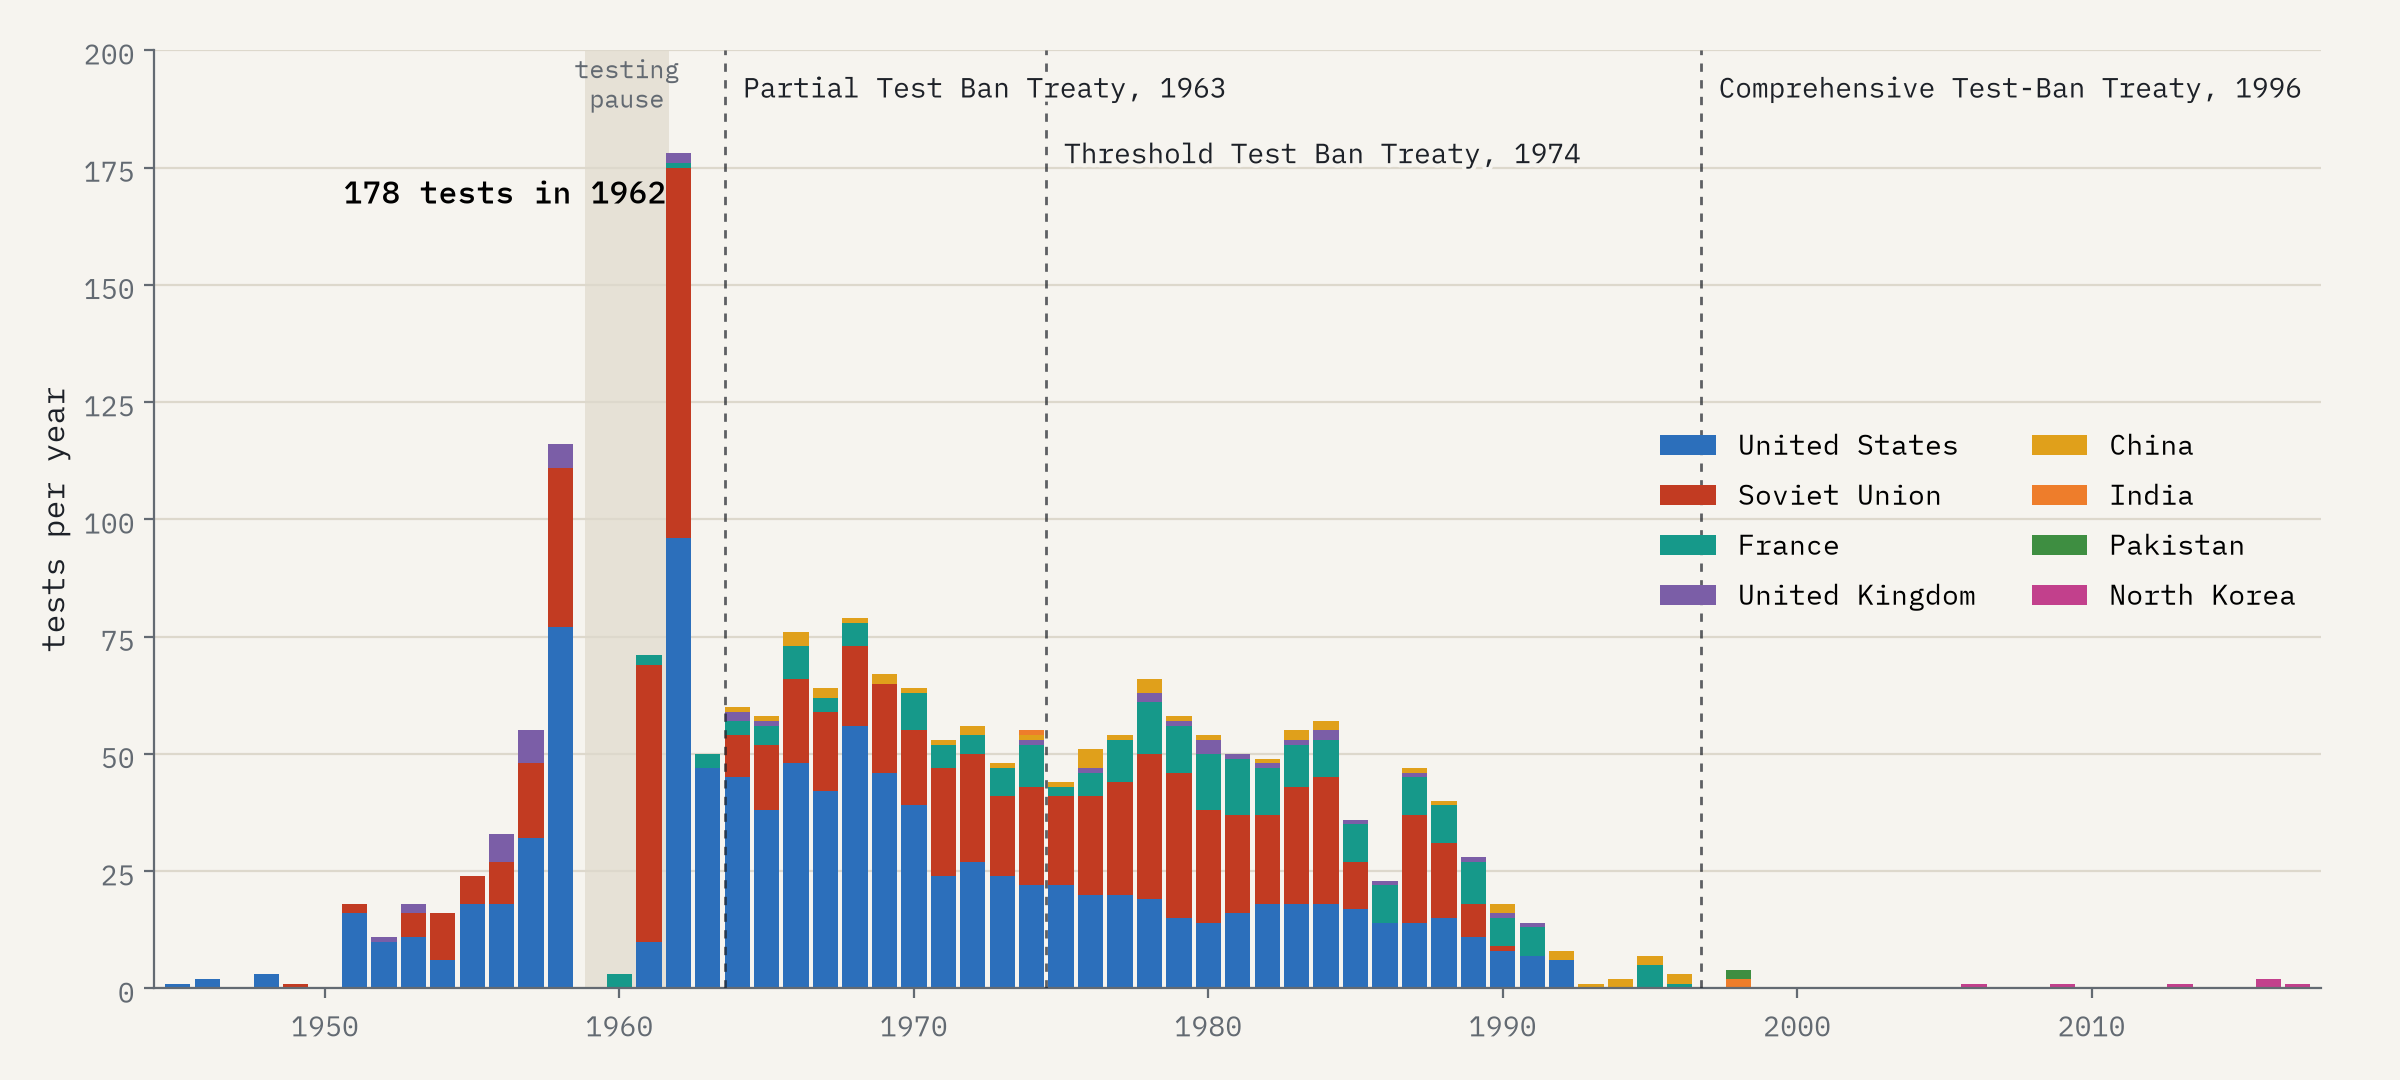
\includegraphics[width=\textwidth]{f_years.png}
\caption{Nuclear tests per year by country, 1945 to 2017, with the 1958 to 1961 testing pause and the treaties of 1963, 1974 and 1996.}\label{fig:years}\end{figure}

\begin{table}[tbp]\centering\footnotesize\setlength{\tabcolsep}{4pt}\caption{Tests by country: count in this study and in the Wikipedia list, first and last year, atmospheric or underwater and underground tests, and total yield in megatons (central estimate and range).}\label{tab:countries}\begin{tabular}{lrrrrrrrr}\toprule Country & Tests & Wikipedia & First & Last & Air/water & Underground & Yield Mt & Range Mt\\\midrule
United States & 1,030 & 1,032 & 1945 & 1992 & 215 & 815 & 200.7 & 168.5 to 232.9\\
Soviet Union & 714 & 727 & 1949 & 1990 & 219 & 495 & 301.4 & 232.4 to 370.5\\
France & 210 & 215 & 1960 & 1996 & 50 & 160 & 12.9 & 2.2 to 23.5\\
United Kingdom & 45 & 88 & 1952 & 1991 & 21 & 24 & 9.6 & 8.4 to 10.8\\
China & 45 & 47 & 1964 & 1996 & 23 & 22 & 21.4 & 16.9 to 25.9\\
India & 3 & 2 & 1974 & 1998 & 0 & 3 & 0.021 & 0.000 to 0.041\\
Pakistan & 2 & 2 & 1998 & 1998 & 0 & 2 & 0.026 & 0.000 to 0.053\\
North Korea & 6 & 6 & 2006 & 2017 & 0 & 6 & 0.2 & 0.1 to 0.3\\
\midrule Total & 2,055 & 2,121 & 1945 & 2017 & 528 & 1,527 & 546.3 & 428.5 to 664.0\\\bottomrule\end{tabular}\end{table}

\subsection{Into the ground}
Before the Partial Test Ban Treaty was signed on 5 August 1963, 459 of 581 tests (79\%) were atmospheric or underwater; after it, 95\% of 1,474 were underground (Figure~\ref{fig:env}). All 69 later atmospheric tests were by the two nuclear states that did not sign: France (46, in French Polynesia, until 1974) and China (23, at Lop Nur, until 1980). The last atmospheric test was Chinese, on 16 October 1980. In all, 528 tests (25.3\% plus 8 underwater) were in the open, but they carried 82\% of the total yield. After the Threshold Test Ban Treaty limit of 150 kilotons took effect in 1976, none of the 517 American and Soviet tests had an upper yield estimate above 150 kilotons.

\begin{figure}[tbp]\centering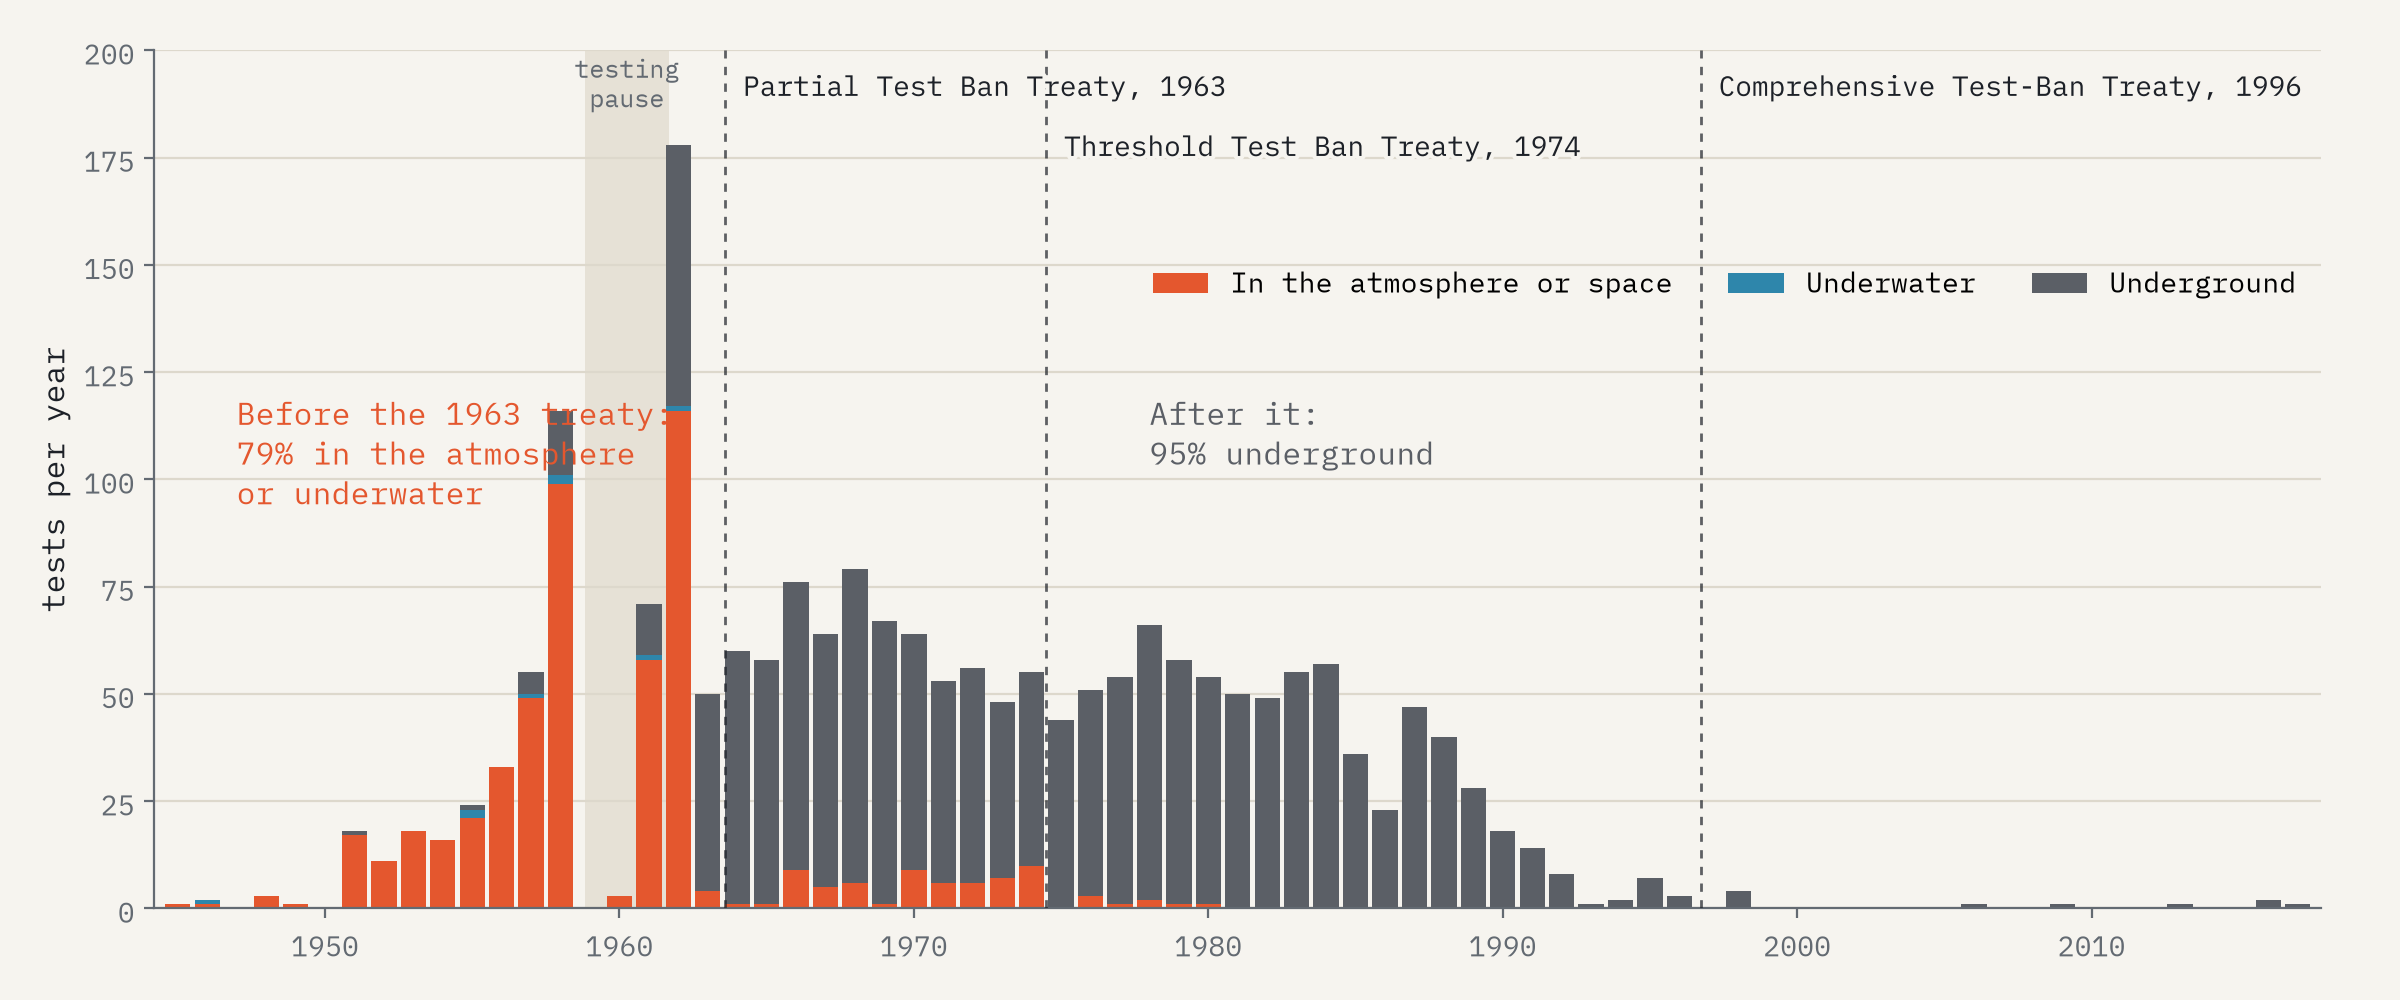
\includegraphics[width=\textwidth]{f_env.png}
\caption{Tests per year by where the device went off: in the atmosphere or space, underwater, or underground.}\label{fig:env}\end{figure}

\subsection{How big}
Yield is concentrated in time, place and a few tests. The median test was 10 kilotons and 65\% had an upper estimate of 20 kilotons or less, but the 85 tests of one megaton or more carry 80\% of the total. The Soviet Union and the United States account for 92\% of the yield. By site (Figure~\ref{fig:yield}), Novaya Zemlya took 51\% of all test yield in 130 tests (93\% of the Soviet total), followed by Bikini Atoll (14.1\%) and the Nevada Test Site (8.4\%), which hosted 45\% of all tests.

\begin{figure}[tbp]\centering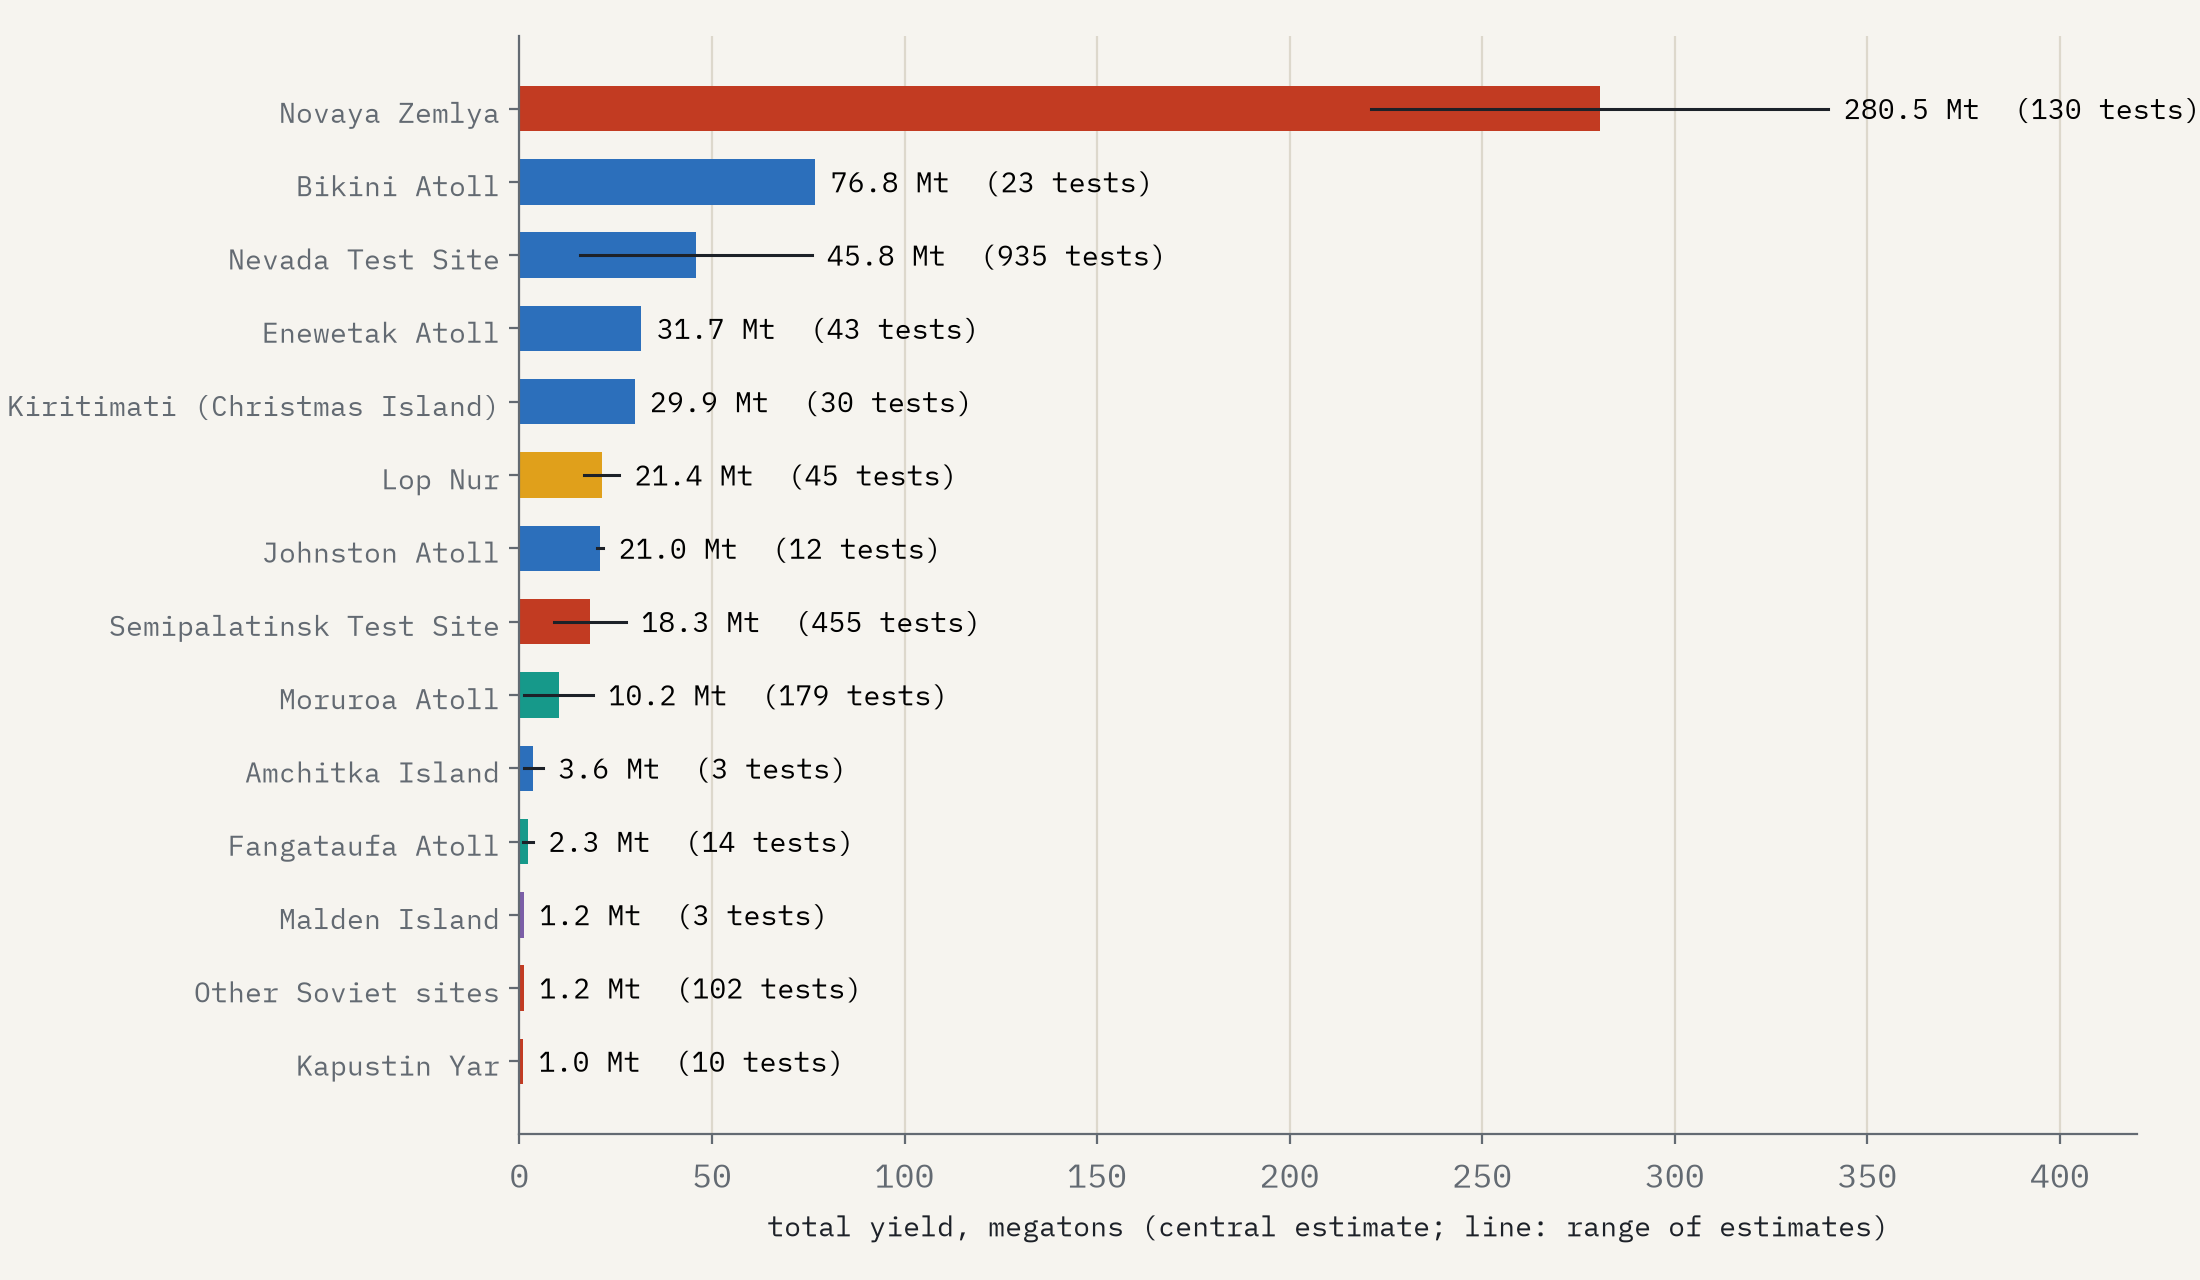
\includegraphics[width=\textwidth]{f_yield.png}
\caption{Total yield by test site: central estimate with the range from the sums of lower and upper estimates.}\label{fig:yield}\end{figure}

\subsection{The biggest tests}
The largest was the Soviet test known as Tsar Bomba, an air drop over Novaya Zemlya on 30 October 1961, at about 50 megatons, 9.2\% of all test yield. Of the twenty largest tests (Figure~\ref{fig:biggest}), 11 were Soviet and 9 American, and 12 took place in 1961 or 1962. The SIPRI list gives the Soviet test of 27 September 1962 a range of 10 to 50 megatons; its midpoint puts it second here, while Wikipedia gives 20 megatons. The largest American test, Castle Bravo at Bikini on 1 March 1954 local time, yielded 15 megatons; its fallout reached the inhabited Rongelap and Rongerik atolls, which were evacuated, and the crew of the Japanese fishing boat Daigo Fukuryū Maru \citep{wikilist}.

\begin{figure}[tbp]\centering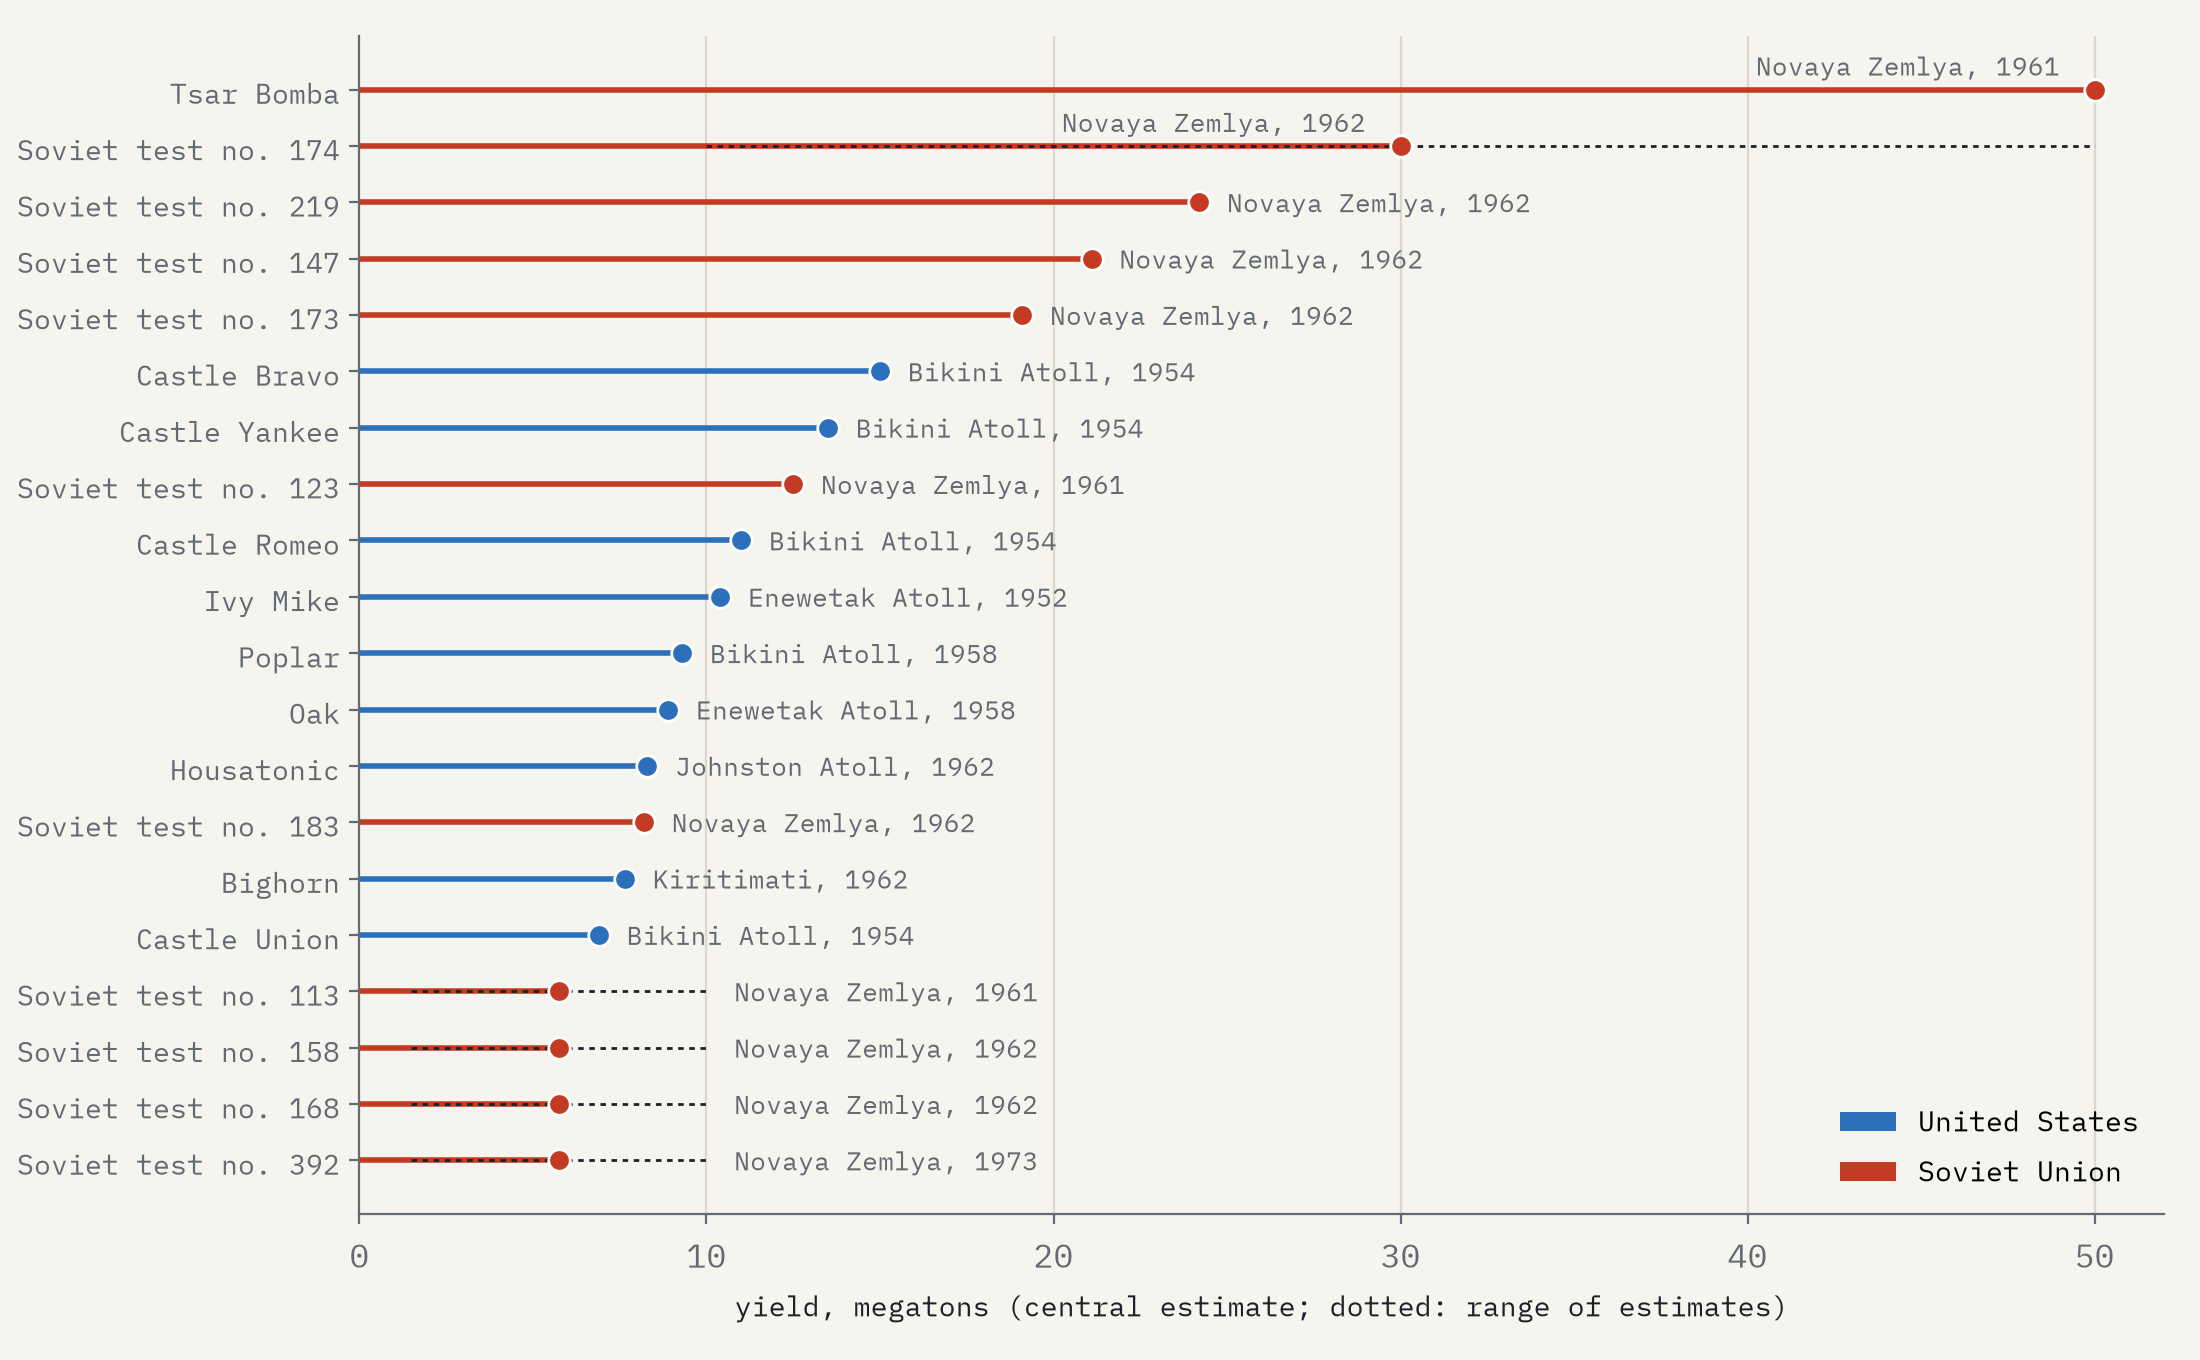
\includegraphics[width=\textwidth]{f_biggest.png}
\caption{The twenty largest nuclear tests by central yield estimate, with the source's range where it gives one.}\label{fig:biggest}\end{figure}

\subsection{Whose land}
82\% of tests were on the testing state's own national territory, but these carried 68\% of the yield (Figure~\ref{fig:land}). 297 tests (14\%) were in the testing state's colonies, overseas territories or trust territories, with 27\% of the yield, and 60 (3\%) on another state's territory or colony. Every French test (210) and every British test (45) was outside the testing state's home territory.

France tested 17 times in the Algerian Sahara from 1960 to 1966, four times in the atmosphere at Reggane during the war of independence; 11 of its underground tests at In Ekker took place after Algeria became independent on 5 July 1962. It then moved to Moruroa and Fangataufa in French Polynesia, where it carried out 193 tests from 1966 to 1996, 46 of them atmospheric. Britain tested 12 times in Australia from 1952 to 1957, including at Maralinga and Emu Field on Aboriginal lands \citep{royal}; 9 times on Malden Island and Kiritimati, then British-held and now part of Kiribati; and 24 times in Nevada. The United States held 66 tests at Bikini and Enewetak in the Marshall Islands from 1946 to 1958, a UN trust territory under US administration from 1947, whose people were moved before the tests \citep{unscear}; they released 20\% of all test yield and 54\% of the American total. The Soviet Union and China tested only within their own borders, at sites that lay in the Kazakh Soviet republic, in the Russian Arctic, where the Nenets residents of Novaya Zemlya were relocated \citep{khalturin}, and in Xinjiang. The Nevada Test Site lies on land the Western Shoshone claim under the Treaty of Ruby Valley \citep{kuletz}.

Islands carried most of the yield: 440 tests (21\%) were on islands and atolls, but they released 84\% of all test yield and 94\% of the atmospheric yield. The Pacific atolls of Bikini, Enewetak, Johnston, Kiritimati, Malden, Moruroa and Fangataufa together saw 304 tests and 32\% of the yield.

\begin{figure}[tbp]\centering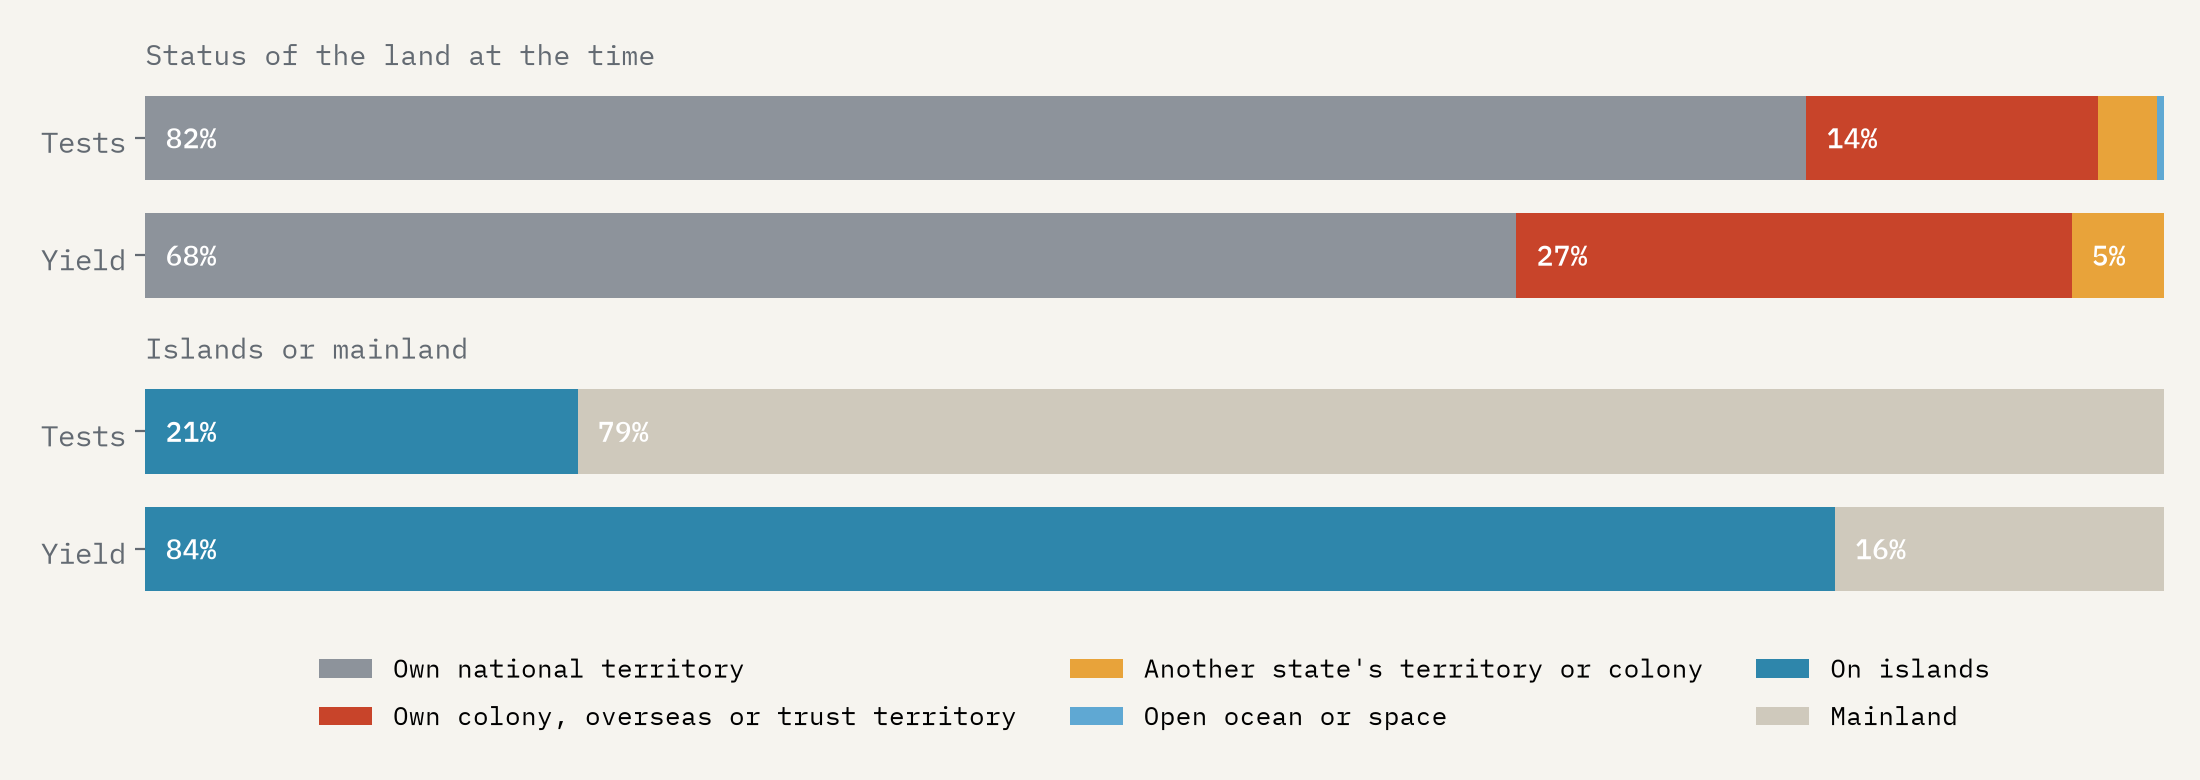
\includegraphics[width=\textwidth]{f_land.png}
\caption{Share of tests and yield by the status of the land at the time of the test, and on islands against the mainland.}\label{fig:land}\end{figure}

{\footnotesize\begin{longtable}{p{3.3cm}rp{1.2cm}rp{2.2cm}p{5.6cm}}\caption{Test sites: tests, years, total yield (megatons, central estimate), status of the land at the time (for the testing state that used it most) and notes. Sources in brackets; see the reference list.}\label{tab:sites}\\\toprule Site & Tests & Years & Yield & Land & Note\\\midrule\endfirsthead\toprule Site & Tests & Years & Yield & Land & Note\\\midrule\endhead
\textbf{Nevada Test Site and nearby ranges}, Nevada, United States & 935 & 1951 to 1992 & 45.8 & Own national territory & The main US test site from 1951 to 1992, in the desert north of Las Vegas, on land the Western Shoshone claim under the 1863 Treaty of Ruby Valley (Kuletz 1998). 24 British tests were also held here. Fallout from the atmospheric tests of the 1950s drifted over communities downwind (UNSCEAR 2000).\\
\textbf{Semipalatinsk Test Site}, Kazakhstan & 455 & 1949 to 1989 & 18.3 & Own national territory & The main Soviet test site, on the steppe of the Kazakh Soviet republic, used from 1949 to 1989. People living in villages nearby were exposed to fallout from the early tests (UNSCEAR 2000). Kazakhstan closed the site on 29 August 1991, the date the United Nations now marks as the International Day against Nuclear Tests.\\
\textbf{Moruroa Atoll}, French Polynesia & 179 & 1966 to 1995 & 10.2 & Own colony, overseas or trust territory & An atoll in French Polynesia, then a French overseas territory: 179 tests from 1966 to 1995, in the atmosphere until 1974, then underground (Wikipedia). In 2010 France passed a law to compensate people made ill by its tests.\\
\textbf{Novaya Zemlya}, Arctic Russia & 130 & 1955 to 1990 & 280.5 & Own national territory & An Arctic archipelago. Its small Nenets population was moved to the mainland when the test site was set up in the mid 1950s (Khalturin et al. 2005). Tsar Bomba and almost all of the largest Soviet tests were fired here: 93\% of all Soviet test yield.\\
\textbf{Other Soviet sites (mostly peaceful explosions)}, Russia, Kazakhstan, Ukraine, Uzbekistan and Turkmenistan & 102 & 1954 to 1988 & 1.2 & Own national territory & Peaceful nuclear explosions across Russia, Kazakhstan, Ukraine, Uzbekistan and Turkmenistan, for seismic surveys, gas and oil work and underground cavities, and a 1954 military exercise in the Orenburg region (SIPRI purposes).\\
\textbf{Lop Nur}, Xinjiang, China & 45 & 1964 to 1996 & 21.4 & Own national territory & China's only test site, in the desert of Xinjiang, used from 1964 to 1996: 23 tests in the atmosphere, the last in 1980, then underground (Wikipedia).\\
\textbf{Enewetak Atoll}, Marshall Islands & 43 & 1948 to 1958 & 31.7 & Own colony, overseas or trust territory & Marshall Islands, a UN trust territory administered by the United States. Its people were moved to Ujelang Atoll in 1947 (UNSCEAR 2000). Ivy Mike, the first full scale hydrogen bomb, was fired here in 1952.\\
\textbf{Kiritimati (Christmas Island)}, Kiribati & 30 & 1957 to 1962 & 29.9 & Own colony, overseas or trust territory & Then part of a British colony in the central Pacific, now Kiribati. Britain tested hydrogen bombs here in 1957 and 1958, and the United States fired 24 air drops nearby in 1962 (Wikipedia).\\
\textbf{Bikini Atoll}, Marshall Islands & 23 & 1946 to 1958 & 76.8 & Own colony, overseas or trust territory & In the Marshall Islands, from 1947 a UN trust territory administered by the United States. Its people were moved off before the first tests in 1946 (UNSCEAR 2000). Fallout from Castle Bravo in 1954 reached the inhabited Rongelap and Rongerik atolls, which were evacuated (Wikipedia).\\
\textbf{Azgir}, Kazakhstan & 17 & 1966 to 1979 & 0.5 & Own national territory & Peaceful explosions in salt domes in western Kazakhstan, to make underground cavities.\\
\textbf{Fangataufa Atoll}, French Polynesia & 14 & 1966 to 1996 & 2.3 & Own colony, overseas or trust territory & Moruroa's neighbouring atoll in French Polynesia: France's first hydrogen bomb, Canopus, in 1968, and its last test, in January 1996 (Wikipedia).\\
\textbf{In Ekker}, Algeria & 13 & 1961 to 1966 & 0.3 & Own colony, overseas or trust territory & Underground tests in the Hoggar mountains of the Algerian Sahara, 1961 to 1966. 11 of the 13 took place after Algeria became independent on 5 July 1962, under the Evian Accords.\\
\textbf{Johnston Atoll}, Central Pacific (US territory) & 12 & 1958 to 1962 & 21.0 & Own colony, overseas or trust territory & A small US-held atoll in the central Pacific with no permanent population, used for high altitude rocket shots in 1958 and 1962.\\
\textbf{Kapustin Yar}, Astrakhan region, Russia & 10 & 1957 to 1962 & 1.0 & Own national territory & A missile range near the Volga, used for rocket-carried and high altitude tests from 1957 to 1962.\\
\textbf{Open ocean (Pacific and South Atlantic)}, High seas & 7 & 1955 to 1962 & 0.046 & Open ocean or space & Shots fired far from land, over or under the open Pacific and, in 1958, high above the South Atlantic.\\
\textbf{Maralinga}, South Australia & 7 & 1956 to 1957 & 0.061 & Another state's territory or colony & Seven British tests in 1956 and 1957 on the traditional lands of the Maralinga Tjarutja, an Anangu people. A Royal Commission reported on the British tests and their effects on Aboriginal people in 1985; the last of the test lands were handed back to the Maralinga Tjarutja in 2014.\\
\textbf{Other US mainland sites}, New Mexico, Colorado and Mississippi, United States & 6 & 1961 to 1973 & 0.1 & Own national territory & Peaceful and research explosions: gas well stimulation in New Mexico and Colorado, and shots in salt in New Mexico and Mississippi (SIPRI purposes).\\
\textbf{Punggye-ri}, North Hamgyong, North Korea & 6 & 2006 to 2017 & 0.2 & Own national territory & North Korea's six tests, 2006 to 2017, all underground in tunnels at Punggye-ri in the mountains of the north east. Yields are estimates, given as ranges (Wikipedia).\\
\textbf{Reggane}, Algeria & 4 & 1960 to 1961 & 0.1 & Own colony, overseas or trust territory & In the Algerian Sahara, then under French colonial rule and during the Algerian war of independence: France's first four tests, in the atmosphere, 1960 and 1961 (Wikipedia).\\
\textbf{Amchitka Island}, Aleutian Islands, Alaska, United States & 3 & 1965 to 1971 & 3.6 & Own national territory & Three underground tests in the Aleutian Islands of Alaska, including Cannikin in 1971, the largest US underground test (Wikipedia).\\
\textbf{Malden Island}, Kiribati & 3 & 1957 & 1.2 & Own colony, overseas or trust territory & An uninhabited British-held island in the central Pacific, now part of Kiribati: Britain's first hydrogen bomb trials, 1957 (Wikipedia).\\
\textbf{Montebello Islands}, Western Australia & 3 & 1952 to 1956 & 0.1 & Another state's territory or colony & Uninhabited islands off Western Australia: Britain's first atomic test, Hurricane, in 1952, fired in a ship (Wikipedia).\\
\textbf{Pokhran}, Rajasthan, India & 3 & 1974 to 1998 & 0.021 & Own national territory & India's test range in the Thar Desert of Rajasthan: Smiling Buddha in 1974 and the five devices of Pokhran-II in 1998. The range itself is uninhabited, but houses in villages within five kilometres were damaged (Wikipedia).\\
\textbf{Emu Field}, South Australia & 2 & 1953 & 0.018 & Another state's territory or colony & Two British tests in the South Australian desert in 1953, on the lands of Anangu Aboriginal people (Royal Commission 1985).\\
\textbf{Trinity, Alamogordo}, New Mexico, United States & 1 & 1945 & 0.021 & Own national territory & The first nuclear test, on 16 July 1945, on the Alamogordo bombing range in the New Mexico desert.\\
\textbf{Ras Koh Hills, Chagai}, Balochistan, Pakistan & 1 & 1998 & 0.018 & Own national territory & Chagai-I, Pakistan's first tests: five devices fired together inside a mountain in the Ras Koh Hills of Balochistan on 28 May 1998 (Wikipedia).\\
\textbf{Kharan Desert}, Balochistan, Pakistan & 1 & 1998 & 0.009 & Own national territory & Chagai-II, Pakistan's second test, in the Kharan Desert of Balochistan on 30 May 1998 (Wikipedia).\\
\bottomrule\end{longtable}}

\subsection{After 1996}
The Comprehensive Nuclear-Test-Ban Treaty opened for signature on 24 September 1996 and has not entered into force. The last tests of the United States (23 September 1992), the Soviet Union (24 October 1990), the United Kingdom (26 November 1991), France (27 January 1996) and China (29 July 1996) came before it. Since then there have been 10 tests: two by India and two by Pakistan in May 1998 and six by North Korea from 2006 to 2017 (Figure~\ref{fig:nk}), whose estimated yields total 101 to 345 kilotons.

\begin{figure}[tbp]\centering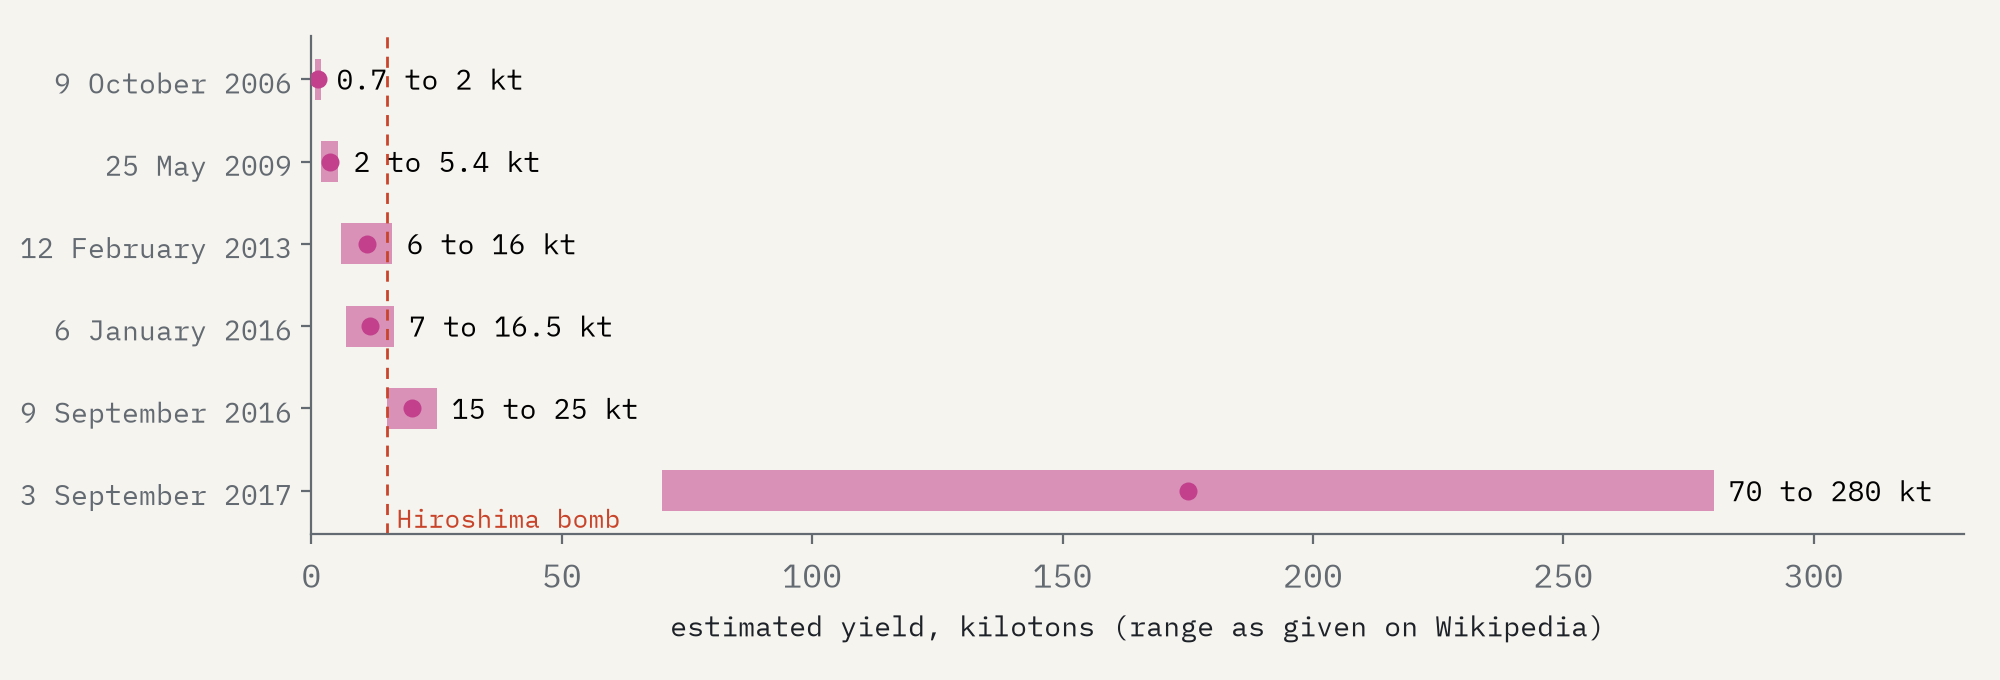
\includegraphics[width=.9\textwidth]{f_nk.png}
\caption{North Korea's six tests: estimated yield ranges as given on Wikipedia, with the Hiroshima bomb for scale.}\label{fig:nk}\end{figure}

\section{Limitations}
The SIPRI list ends in 1998 and the North Korean records come from a tertiary source. Yields are estimates, many of them only upper bounds, and the central estimates for small tests are rough; the totals are dominated by large tests whose yields are better known. Counts depend on how salvoes, safety trials and failed tests are treated. Positions are as recorded, rounded in many cases, and 24 are approximate. The classification of land is a simple description of status at the time and does not capture the full history or present claims of the peoples concerned. Above all, this is a map of explosions, not of exposure or harm: fallout travelled far beyond the sites, and its effects on local populations and test personnel are studied elsewhere \citep{unscear}.

\section{Conclusion}
Nuclear testing was frequent, then hidden, then nearly over. Most tests were small and underground, on the testing state's own soil. But most of the energy released came from a few dozen atmospheric tests in the 1950s and early 1960s, set off over Arctic islands and Pacific atolls and in colonial and trust territories far from the governments that ordered them.

\section*{Data and code availability}
The interactive map is at \url{https://maps.tristanhotham.com/nuclear-tests/}. Data and code are at \url{https://github.com/Tristan-Hotham/nuclear-tests} and archived with this paper at https://doi.org/10.5281/zenodo.23857489. Derived data are released under CC BY 4.0 and code under the MIT licence, except material derived from Wikipedia (the North Korean records, test names and site notes drawing on Wikipedia), which is shared under CC BY-SA 4.0.

\section*{AI statement}
I wrote the text, with drafting and editing assistance from Claude (Anthropic), which also helped prepare the analysis code. I reviewed and checked all text and results.

\begin{thebibliography}{99}
\bibitem[Bergkvist and Ferm(2000)]{sipri} Bergkvist, N.-O. and Ferm, R. (2000) \emph{Nuclear Explosions 1945 to 1998}. Stockholm: Swedish Defence Research Establishment (FOA) and Stockholm International Peace Research Institute (SIPRI).
\bibitem[Khalturin et al.(2005)]{khalturin} Khalturin, V. I., Rautian, T. G., Richards, P. G. and Leith, W. S. (2005) A review of nuclear testing by the Soviet Union at Novaya Zemlya, 1955 to 1990. \emph{Science and Global Security} 13: 1 to 42.
\bibitem[Kuletz(1998)]{kuletz} Kuletz, V. L. (1998) \emph{The Tainted Desert: Environmental and Social Ruin in the American West}. New York: Routledge.
\bibitem[Mikhailov(1996)]{mikhailov} Mikhailov, V. N. (ed.) (1996) \emph{USSR Nuclear Weapons Tests and Peaceful Nuclear Explosions, 1949 through 1990}. Sarov: RFNC-VNIIEF.
\bibitem[Natural Earth(2026)]{naturalearth} Natural Earth (2026) Admin 0 countries and populated places. Public domain. \url{https://www.naturalearthdata.com/}
\bibitem[Royal Commission(1985)]{royal} Royal Commission into British Nuclear Tests in Australia (1985) \emph{Report}. Canberra: Australian Government Publishing Service.
\bibitem[TidyTuesday(2019)]{tidytuesday} R for Data Science Online Learning Community (2019) TidyTuesday, 20 August 2019: Nuclear Explosions. \url{https://github.com/rfordatascience/tidytuesday/tree/main/data/2019/2019-08-20}; from data is plural, \url{https://github.com/data-is-plural/nuclear-explosions}; credit Jesus Castagnetto.
\bibitem[UNSCEAR(2000)]{unscear} United Nations Scientific Committee on the Effects of Atomic Radiation (2000) \emph{Sources and Effects of Ionizing Radiation}, Annex C: Exposures to the public from man-made sources of radiation. New York: United Nations.
\bibitem[US DOE(2015)]{doe} US Department of Energy, National Nuclear Security Administration (2015) \emph{United States Nuclear Tests, July 1945 through September 1992}. DOE/NV-209, revision 16.
\bibitem[Wikipedia(2026a)]{wikilist} Wikipedia contributors (2026) List of nuclear weapons tests. Revision 1378389080. CC BY-SA 4.0. \url{https://en.wikipedia.org/wiki/List_of_nuclear_weapons_tests}
\bibitem[Wikipedia(2026b)]{wikink} Wikipedia contributors (2026) List of nuclear weapons tests of North Korea. Revision 1378498359. CC BY-SA 4.0. \url{https://en.wikipedia.org/wiki/List_of_nuclear_weapons_tests_of_North_Korea}
\bibitem[Wikipedia(2026c)]{wikipok} Wikipedia contributors (2026) Pokhran-II. Revision 1376678335. CC BY-SA 4.0. \url{https://en.wikipedia.org/wiki/Pokhran-II}
\bibitem[Wikipedia(2026d)]{wikichagai} Wikipedia contributors (2026) Chagai-I. Revision 1370612927. CC BY-SA 4.0. \url{https://en.wikipedia.org/wiki/Chagai-I}
\end{thebibliography}
\end{document}
